\documentclass[sigconf,authorversion,nonacm]{acmart}
\settopmatter{printacmref=false}
\setcopyright{none}
\usepackage{booktabs}
\usepackage{tikz}

\title{Finding the Right Moment: Evidence-Grounded Medical Video Question Answering with Medix}
\author{Author information to be supplied}

\begin{document}
\begin{abstract}
Someone seeking help with a medical procedure may need a short answer tied to the right part of a video. Finding a plausible video is only the first step. Medix retrieves videos, finds a relevant time interval, collects evidence, and can produce a short answer that cites its source. We evaluate this pipeline on the video-disjoint MedVidQA benchmark. The catalog contains 852 available videos. On 155 test questions, the correct video appears in the top five for 88 (56.8\%). The complete pipeline builds evidence for 56 questions (36.1\%), selects the correct video for 27 (17.4\%), and finds a correct-video interval with temporal intersection-over-union at least 0.5 for eight (5.2\%). An extractive answer is produced for 54 questions. Its 148 claims all reproduce cited transcript text, but this check does not show that the answers are medically correct. A separate confidence experiment uses a different retrieval task and cannot establish an end-to-end gain. The large drop between video retrieval and usable evidence shows where this prototype needs improvement before its guidance can be trusted.
\end{abstract}

\maketitle

\section{Introduction}
A person asking how to perform a procedure may have little time or a free hand to search a long video. Medix is motivated by that setting: it aims to find a useful moment and present short guidance with a visible source. This study tests the evidence-finding pipeline, not a hands-free device or its effect on care. A fluent answer can still come from the wrong video, the wrong moment, or an irrelevant transcript cue. MedVidQA provides expert questions and annotated answer intervals, so we can measure video retrieval and temporal localization \cite{gupta2023medvidqa}. It does not label the medical correctness of generated instructions.

We ask: \emph{How often does a retrieved medical video lead to evidence from the correct moment?} We then ask whether video frames help locate that moment when the correct video is already known. Finally, we ask what a source-citing answer can prove when no reference answer or clinical judgment is available. Figure~\ref{fig:pipeline} shows the stages we test.

Our contribution is a stage-by-stage audit on the official validation and test splits. We report how much media is available, how each stage performs, and how the full pipeline performs without the correct video or interval as input. We also separate an early confidence-model experiment because it uses a different retrieval index. These results evaluate a prototype; they do not establish safe medical advice.

\begin{figure}[t]
\centering
\setlength{\fboxsep}{3pt}
\begin{tabular}{c}
\fbox{\parbox{.81\columnwidth}{\centering Medical procedure question}}\\[-2pt]
$\downarrow$\\[-2pt]
\fbox{\parbox{.81\columnwidth}{\centering Retrieve five videos from title and author}}\\[-2pt]
$\downarrow$\\[-2pt]
\fbox{\parbox{.81\columnwidth}{\centering Locate a time interval using transcript and frames}}\\[-2pt]
$\downarrow$\\[-2pt]
\fbox{\parbox{.81\columnwidth}{\centering Build a timestamped evidence bundle or abstain}}\\[-2pt]
$\downarrow$\\[-2pt]
\fbox{\parbox{.81\columnwidth}{\centering Extractive answer with cited transcript cues}}
\end{tabular}
\caption{The evaluated Medix path. The benchmark's annotated video and interval are used only to score predictions. Missing media can stop the path before an answer is produced.}
\Description{Five boxes show a question flowing through video retrieval, interval localization, evidence extraction or abstention, and an extractive answer with cited transcript cues.}
\label{fig:pipeline}
\end{figure}

\section{Related Work}
MedVidQA introduced medical instructional video classification and medical visual answer localization with timestamped intervals \cite{gupta2023medvidqa}. The 2022 shared task compared subtitle- and vision-based localization strategies \cite{gupta2022sharedtask}; the 2024 TREC track extended the research setting to corpus-level video retrieval and query-focused step captions, and used human assessment for generated output \cite{gupta2024trecmedvidqa}. The present evaluation uses the original MedVidQA splits and adds a title-based corpus retrieval stage. Its scores should not be compared directly with systems that are handed the correct video or with the distinct 2024 track data and judgments.

Retrieval-augmented generation conditions a response on an external evidence source \cite{lewis2020rag}. Medical RAG benchmarks show that corpus and retriever selection affect medical QA results \cite{xiong2024medrag}. ASTRID separates context relevance, refusal accuracy, and conversational faithfulness in clinical RAG evaluation \cite{he2025astrid}. Those studies motivate distinct outcomes for finding a source, deciding to answer, and checking claims. In Medix, a valid cue ID establishes a link to source text; it does not prove entailment, completeness, or clinical appropriateness. We therefore refrain from a novelty claim over all medical video assistants until a broader literature search, specified in the companion research agenda, is completed.

\section{Data}
\subsection{Benchmark and observable media}
The official MedVidQA files contain 2,710 training, 145 validation, and 155 test questions (Table~\ref{tab:data}). Their videos are disjoint across splits: 800, 49, and 50 videos, respectively. Each question has a video ID and an annotated answer interval. We use the original validation and test splits. A separate cleaned copy removes 144 of 3,010 questions, but its results are not mixed into this analysis.

\begin{table}[t]
\caption{Official data and local evidence availability. Coverage is a property of this cache and acquisition process, not of the original dataset.}
\label{tab:data}
\centering
\begin{tabular}{lrrr}
\toprule
 & Train & Validation & Test \\
\midrule
Questions & 2,710 & 145 & 155 \\
Distinct videos & 800 & 49 & 50 \\
Questions with cached transcript & -- & 76 & 69 \\
Questions with local visual evidence & -- & 75 & 67 \\
\bottomrule
\end{tabular}
\end{table}

Each catalog record contains a video title, optional author, URL, and duration. It contains no benchmark question or answer interval. Metadata collection produced 852 records and failed for 47 video IDs. The correct video is present for 143/155 test questions. Cached transcripts cover 69/155, and local video frames cover 67/155. We count missing media as failures on the full test set. Because caption and video availability are uneven, results on the covered subset may not represent the full dataset.

\subsection{Outcome definitions}
Recall@\(k\) asks whether the correct video appears in the first \(k\) results. Mean reciprocal rank (MRR) rewards placing it higher. Temporal intersection-over-union (IoU) measures how much the predicted time interval overlaps the annotated interval. A missing interval or wrong video scores zero. We report the fraction with a correct video and IoU at least \(\tau\) as \(R@1,\operatorname{IoU}\geq\tau\). We also report how often the system builds a complete evidence bundle, selects the correct video, and answers. These measures test different steps; none measures medical correctness.

\section{Methods}
\subsection{Video retrieval and temporal localization}
The retriever represents each question and catalog record with \texttt{all-MiniLM-L6-v2}. Its score blends embedding similarity and title/author word overlap: \(0.85s_{\rm dense}+0.15s_{\rm lexical}\). It keeps five videos. The recorded run uses this weight; there is no documented validation search for it. We calculate an expected uniform-random Recall@5 as a reference, not as the result of repeated random trials.

We first test localization with the correct video supplied. The transcript is cut into overlapping windows and each window is matched to the question. Validation compared window lengths of 15, 30, 45, 60, and 90 seconds. It selected 90-second windows with a 45-second stride. A second model samples three frames per window and scores them with CLIP. Validation selected equal transcript and visual weights from the tested transcript weights 0, 0.25, 0.5, and 0.75. If frames are missing, the model uses the transcript alone. Random Mode and Random Guess provide temporal references. We compare text and visual methods on the same visually covered test questions. This diagnostic gives the model the correct video, so it is easier than the full task.

\subsection{End-to-end selection and grounded output}
In the full task, the runner receives only a question. It retrieves five videos and tries to find a relevant interval in each available transcript and frame set. It ranks candidates that can yield a complete bundle containing transcript text, sampled frames, and a clip. If none can, it abstains. Validation selected a retrieval weight of zero for the final candidate score, using mean end-to-end IoU. Retrieval still matters: the correct video must first reach the top five. The test run uses this selected setting. Correct video IDs and intervals are revealed only for scoring. An older validation file uses a weight of 0.5 and is not the selected run.

The offline answer baseline picks up to three transcript cues using word overlap with the question and copies their text into the answer. It cites each cue. The checks reject unknown cue IDs and measure whether claims copy the cited text. Copying makes these provenance checks pass by construction. It does not show whether the cue answers the question or whether the advice is correct. This generation result is separate from localization; it is not a full-test comparison against an unconstrained language model.

\section{Results}
\subsection{A retrieval-to-evidence bottleneck}
The video retriever finds the correct video first for 29.7\% of test questions and within the top five for 56.8\% (88/155). Its mean reciprocal rank is 0.404 among 852 catalog videos. The correct video is absent from the catalog for 12 questions, limiting this retriever to 92.3\% recall even with perfect ranking. Figure~\ref{fig:outcomes} shows the larger loss between finding a candidate and returning the right interval.

\begin{figure}[t]
\centering
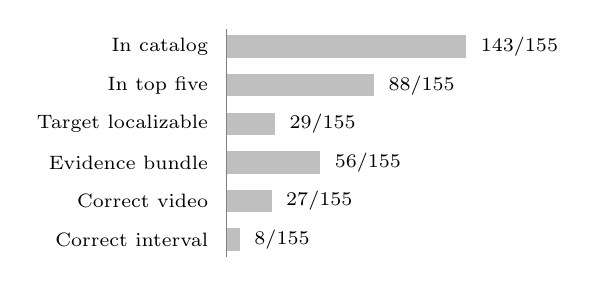
\begin{tikzpicture}[x=1cm,y=.49cm]
\foreach \y/\label/\n/\w in {
5/{In catalog}/143/3.046,
4/{In top five}/88/1.874,
3/{Target localizable}/29/.617,
2/{Evidence bundle}/56/1.191,
1/{Correct video}/27/.574,
0/{Correct interval}/8/.171}
{\node[anchor=east,font=\scriptsize] at (2.05,\y) {\label};
 \fill[black!25] (2.16,\y-.29) rectangle ({2.16+\w},\y+.29);
 \node[anchor=west,font=\scriptsize] at ({2.22+\w},\y) {\n/155};}
\draw[gray] (2.16,-.45) -- (2.16,5.45);
\end{tikzpicture}
\caption{Observed test outcomes (155 questions). Each bar shows the share of all test questions; its label shows the count. These events are not all nested: a complete bundle may come from a wrong video, while ``target localizable'' requires the correct video to be in the top five with a cached transcript. A correct interval requires the correct video and IoU $\geq0.5$.}
\Description{Six bars show counts out of 155 questions: target in catalog 143, target in top five 88, target localizable 29, evidence bundle 56, correct video 27, and correct-video interval at IoU at least 0.5 eight.}
\label{fig:outcomes}
\end{figure}

The full runner builds evidence for 56/155 questions and selects the correct video for 27/155. Thus, 27 of the 56 answered questions (48.2\%) use the right video. Mean IoU is 0.052. The shares with a correct-video interval at IoU thresholds 0.3, 0.5, and 0.7 are 8.4\%, 5.2\%, and 1.9\%. Of 88 questions whose target reaches the top five, 59 have no cached transcript for that video. Only 29 targets can therefore be localized. Forty-four of those 88 questions receive no bundle, while 29 of the 56 answered questions use a wrong video.

We resampled the 50 test videos, keeping all questions from each sampled video together, 10,000 times. The resulting 95\% percentile intervals are [42.5\%, 71.7\%] for Recall@5, [24.6\%, 48.3\%] for evidence coverage, and [0.6\%, 12.0\%] for a correct-video interval at IoU at least 0.5. They describe variation across videos under the current fixed model and media cache. The recorded mean latency is 1.00 seconds per query for cached retrieval, localization, and extraction; it excludes answer generation and acquiring missing media. Finding a video in the top five is much more common than finding evidence from the right moment.

\subsection{What visual reranking changes}
When given the correct video, the transcript-only method reaches mean IoU 0.115 and correct-video IoU-at-least-0.5 recall 9.7\% on all 155 questions. Adding visual frame scores yields 0.129 and 11.6\%. Missing transcripts count as zero. To compare the methods fairly, we also use the same 67 questions with local visual evidence. On this subset, mean IoU rises from 0.257 to 0.289, a gain of 0.032. Recall at IoU at least 0.5 rises from 20.9\% to 25.4\%; random-guess mean IoU is 0.145. A paired bootstrap over the subset's 19 videos gives a 95\% interval of [0.000, 0.069] for the mean-IoU gain and [0.0, 11.5] percentage points for the recall gain. Both intervals include zero. The observed improvement is promising but does not establish a reliable advantage. These frames come from instructional videos, not a user's live viewpoint.

\subsection{Generation and an exploratory confidence experiment}
The extractive baseline answers 54/155 questions and emits 148 cited claims. All 148 claims point to valid transcript cues and copy their text. The video is correct for only 27 of the 54 answers. Perfect citation and copying rates follow from the extractive design; they do not show that a copied instruction is relevant or medically correct. A five-case review by two raters compares three answer styles, but the raters disagree substantially and their qualifications are undocumented. This small pilot can refine a review rubric, not support a safety claim.

A separate experiment estimates the probability that the top retrieved \emph{question record} matches the target video. It freezes 2,574/142/150 train/validation/test question-level retrieval records, excludes the query's own sample ID, and compares eight-feature logistic, 331-parameter MLP, and 329-parameter spline-based KAN models over five training seeds. On its 150-example test split, mean Brier scores are 0.1609, 0.1507, and 0.1361, respectively. Averaging predictions across seeds and bootstrapping test examples gives a KAN-minus-MLP Brier difference of \(-0.0157\), 95\% interval \([-0.0266,-0.0042]\). The analogous AUROC interval crosses zero. At a threshold seeking 90\% validation precision, KAN answers 7.9\% of test examples on average, and MLP answers none. Other annotated questions from a held-out video can remain in the question index, so this protocol is not the title-only, one-document-per-video task above. Nor has KAN been shown to improve the complete pipeline. A 20-feature evidence-agreement ablation contains no independent reranker, transcript-support, or visual-procedure signal in its frozen records; its apparent gains do not test multimodal agreement.

\section{Discussion}
\subsection{Interpretation and threats to validity}
The main problem is clear in Figure~\ref{fig:outcomes}: Medix often retrieves a plausible source but rarely returns evidence from the correct moment. Missing media explain much of the loss, yet selection also fails: only 27 of 56 answered questions use the annotated video. The runner abstains when it cannot build a complete bundle. This rule is not calibrated to clinical correctness. We cannot call all 99 unanswered questions appropriate safety refusals, because many fail for lack of cached media.

The validation choices were made on 145 questions. Test data contain 155 questions and 50 videos, so question-level standard errors would understate dependence among questions sharing a video. Confidence intervals should resample by video and pair predictions on the same questions. Caption and video acquisition were incomplete and nonuniform. Because the known-video localization study is conditioned on cached transcripts and the retrieval study uses catalog metadata, the difference between their scores is not a causal measure of visual benefit in the end-to-end system. The title metadata may also reveal a procedure category that a live, ambiguous query would not make obvious. A separate cleaned dataset and legacy question-indexed retrieval results are present but should not be pooled with the official-split pipeline.

The generation labels contain answer intervals, not reference answer text or clinical correctness judgments. Lexical overlap can pass an irrelevant or unsafe instruction, and a visually correct interval can still omit a critical warning. A production front end supports follow-up, image, and voice paths, and small fixed-bundle model comparisons are documented, but no held-out benchmark establishes their effect on the core research questions. Offline operation, headset usability, patient benefit, and action recognition remain unevaluated. Any clinical or participant study would need appropriate domain review and institutional ethics approval.

\subsection{Prioritized experiments}
First, acquire transcripts uniformly for candidate videos and record why media are missing. Compare title-based dense retrieval with BM25, dense-only retrieval, and a validation-selected blend on the same catalog. Test a selection rule that always takes retrieval rank one. Then remove visual scores from the full pipeline and compare the same questions with paired, video-level intervals. Tune any confidence threshold on validation only. Finally, separate failures caused by a missing catalog entry, missing transcript, extraction failure, wrong video, and wrong interval. Figure~\ref{fig:outcomes} reports the present full-test outcomes, but a future failure table should identify each cause directly.

For response quality, assemble an independently reviewed answerability and evidence-entailment set that includes unanswerable and out-of-scope questions. Compare extractive, structured, and free-form conditions on identical evidence, including an LLM-only arm only after its prompts, provider, and review protocol are frozen. Pre-register a primary outcome, obtain two qualified independent ratings, report agreement and adjudication, and estimate paired uncertainty by video. A risk-coverage curve should distinguish infrastructure abstention from an evidence-sufficiency decision. For the KAN hypothesis, build features from the same video catalog, test calibration and risk at fixed coverage, ablate each genuinely observed modality, and measure inference cost. Tables for the main paper should state dataset denominator, conditioning, model selection split, confidence interval, and whether a result is confirmatory or exploratory.

\section{Conclusion}
On 155 MedVidQA test questions, Medix finds the target video in its top five for 88, builds a complete evidence bundle for 56, and returns a correct-video interval at IoU at least 0.5 for eight. Its extractive answers cite their source text, but their medical content has not been independently validated. The study shows where evidence is lost and suggests a small visual localization gain on a covered subset. It does not establish reliable procedural guidance or better patient outcomes. The next steps are uniform media acquisition, stronger baselines, and independent assessment of answer quality.

\bibliographystyle{ACM-Reference-Format}
\bibliography{references}
\end{document}
